\section{The conley index}
We start by defining some needed properties of maps:
\begin{definition}[Cofibration]
    Let $(X,A)$ be a topological pair and $Y$ be a topological space. The pair $(X,A)$ satisfies the \textbf{homotopy extension property with respect to } $Y$, if and only if, we can extend homotopies. In other words, for all $f:X\to Y$ and $H:A\times I\to Y$ with $H(x,0)=f(x)$ there exists a continuous extension $F:X\times I\to Y$ with $F(x,0)=f(x)$. 
    If a pair $(X,A)$ satisfies the homotopy extension property with respect to any topological space $Y$, we call $(X,A)$ a \textbf{cofibered pair} and the inclusion $i:A\hookrightarrow X$ a \textbf{cofibration}.
\end{definition}

\begin{definition} For as topological pair $(N,L)$ define $N/L=N/ \sim$ where $x \sim y $ if $x,y\in L$. In other words we contract $L$ to be one point.
\end{definition}

\begin{remark}
In the proof of the Morse homology theorem we want to talk about the homology of index pairs as relative homology groups $H^{\sing}_i(N,L)$. However, if the inclusion $L\to N$ is a cofibration we have the natural isomorphism $H^{\sing}_i(N,L) \cong H^{\sing}_i(N/L)$. This is proven in \cite{LecturesonMorseHomology} chapter two. To show that something is a cofibration we will use the following fact for metric spaces: 

The pair $(N,L)$, where $L$ is closed in $N$ is a cofibration (respectivly the inclusion), if an in $N$ open neighbourhood $U$ of $L$ exists, such that $L$ is a strong deformation retract of $U$. 

 This is also presented in chapter two of \cite{LecturesonMorseHomology}, by showing that such an inclusion admits a Str\o{}m structure. An example of such a cofibration is the pair $(D^n,\partial D^n)$. Finally, a pair that is homeomorphic to a cofibration is again one.
\end{remark}

\begin{definition}[Compact invariant isolated subset]
    For a flow $\phi_t:M\to M$ on a locally compact metric space we call a subset $S\subseteq M$ \textbf{invariant subspace} if and only if $\phi_t(S)=S$ for all $t\in \R$. For any subset $N\subseteq M$ we define the \textbf{maximal invariant subset}
    \begin{align*}
        I(N)&=\{x\in N|~ \phi_t(x)\in N \forall t\in \R\}\\
        &=\bigcap_{t\in \R} \phi_t(N).
        \end{align*} A \textbf{compact invariant subset} $S$ is called \textbf{isolated}, if a compact neighborhood $N$ exists, such that $I(N)=S$.
\end{definition}
\begin{definition}[Index pairs] \label{def: index pairs}
Let $S$ be an isolated compact invariant subset. A topological pair $(N,L)$ of compact subsets of $M$ where $L\subseteq N$ is called an \textbf{index pair of }S, if it satisfies the following:
\begin{enumerate}
    \item $S=I(\overline{N\setminus L})\subseteq (\mathring{N\setminus L})$.
    \item  $x\in L$ and $\phi_{[0,t]}(x)\subseteq N$ implies that  $\phi_{[0,t]}(x)\subseteq L$. We call $L$ \textbf{positively invariant in } $N$. Here $\phi_{[0,t]}(x)\coloneq\{ \phi_{\tilde{t}}(x)|\tilde{t}\in [0,t]\}$.
    \item For all $x\in N$ such that a $t$ exists, with $\phi_t(x)\not\in N$, there exists a $t'$ with $\phi_{[0,t']}(x)\subseteq N$ and $\phi_{t'}(x)\in L$.
\end{enumerate}
    This definition captures how the flow lines leave the invariant space $S$. Due to the third property we call $L$ the \textbf{exit set}.
\end{definition}


\begin{definition}[Regular index pairs]
We call an index pair $(N,L)$ \textbf{regular} if and only if the inclusion $I: L \hookrightarrow N$ is a cofibration.
\end{definition}
\begin{remark}
One can show that every isolated compact invariant subset admits an index pair. We won't proof this, as we will always explicitly define such invariant sets and therefore we won't need such a general statement. However, two index pairs of the same invariant set turn out to be homotopy equivalent with a homotopy induced by the flow. The regularities needed for the proof are, that $\phi_t:M\to M$ is a flow on a locally compact metric space. Those regularities are clearly given in the case of our Riemannian manifolds. We follow a proof from \cite{LecturesonMorseHomology} which itself is a reformulation from the proof given by Salomon in \cite{SalomonConleyIndex}. In this reformulation the language of the proof is adapted while the main arguments stay the same. This led to some redundant steps and vagueness, that I removed whilst making it more concrete.
\end{remark}
\begin{lemma}\label{lem: index invariants lemma 1}
Let $N$ be an isolating neighborhood for the isolated compact invariant set $S$ and let $U$ be a neighbourhood of $S$. Then there exists a $t>0$ such that for any $x \in M$ we have:
\begin{align*}
\phi_{[-t,t]}(x)\subseteq N  \quad \Rightarrow \quad x\in U.
\end{align*} 
\end{lemma}
\begin{proof}
Lets assume this was false. Then for any $t>0$ there would be a $x$ contradicting the implication. So define $x_n \notin U$ such that $\phi_{[-n,n]}\subseteq N$. Since $\phi_0=\id$ we know that all $x_n\in N$ and therefore by the compactness we would have limit points $x\in \overline{M\setminus U}$, such that $\phi_{\R}(x)\subseteq N$. Since $S$ was isolated we need to conclude that $x\in S \cap \overline{M\setminus U}$. This is our contradiction as $U$ was a neighbourhood of the closed $S$ and therefore without restriction open making $M\setminus U$ already closed.
\end{proof}
\begin{remark}
Notice that if $t$ satisfies the conditions of lemma \ref{lem: index invariants lemma 1} then every $\tilde{t}\geq t$ also does. This helps us in the next lemma:
\end{remark}


\begin{lemma} \label{lem: index invariants lemma 2} Let $(N,L)$ and $(\tilde{N},\tilde{L})$ be index pairs for the isolated invariant set $S$ and choose $T\geq 0$ such that the following implications hold for $t\geq T$:
\begin{align}
\phi_{[-t,t]}(x) \subseteq N\setminus L \quad &\Rightarrow \quad x \in \tilde{N}\setminus \tilde{L}, \label{eq: lemma 2 1st implic}\\
\phi_{[-t,t]}(x) \subseteq  \tilde{N}\setminus \tilde{L} \quad &\Rightarrow \quad x \in N\setminus L. \label{eq: lemma 2 2nd implic}
\end{align}
Then the map:
\begin{align*}
h:N/L \times [T,\infty) & \to \tilde{N}/\tilde{L} \\
([x],t) & \mapsto 
\begin{cases}
[\phi_{3t}(x)] & \text{ if } \phi_{[0,2t]}\subseteq N\setminus L \text{ and } \phi_{[t,3t]}(x)\subseteq \tilde{N}\setminus \tilde{L}\\
[\tilde{L}] & \text{ otherwise,}
\end{cases}
\end{align*}
is continuous.
\end{lemma}
\begin{figure}[p!]
    \centering
    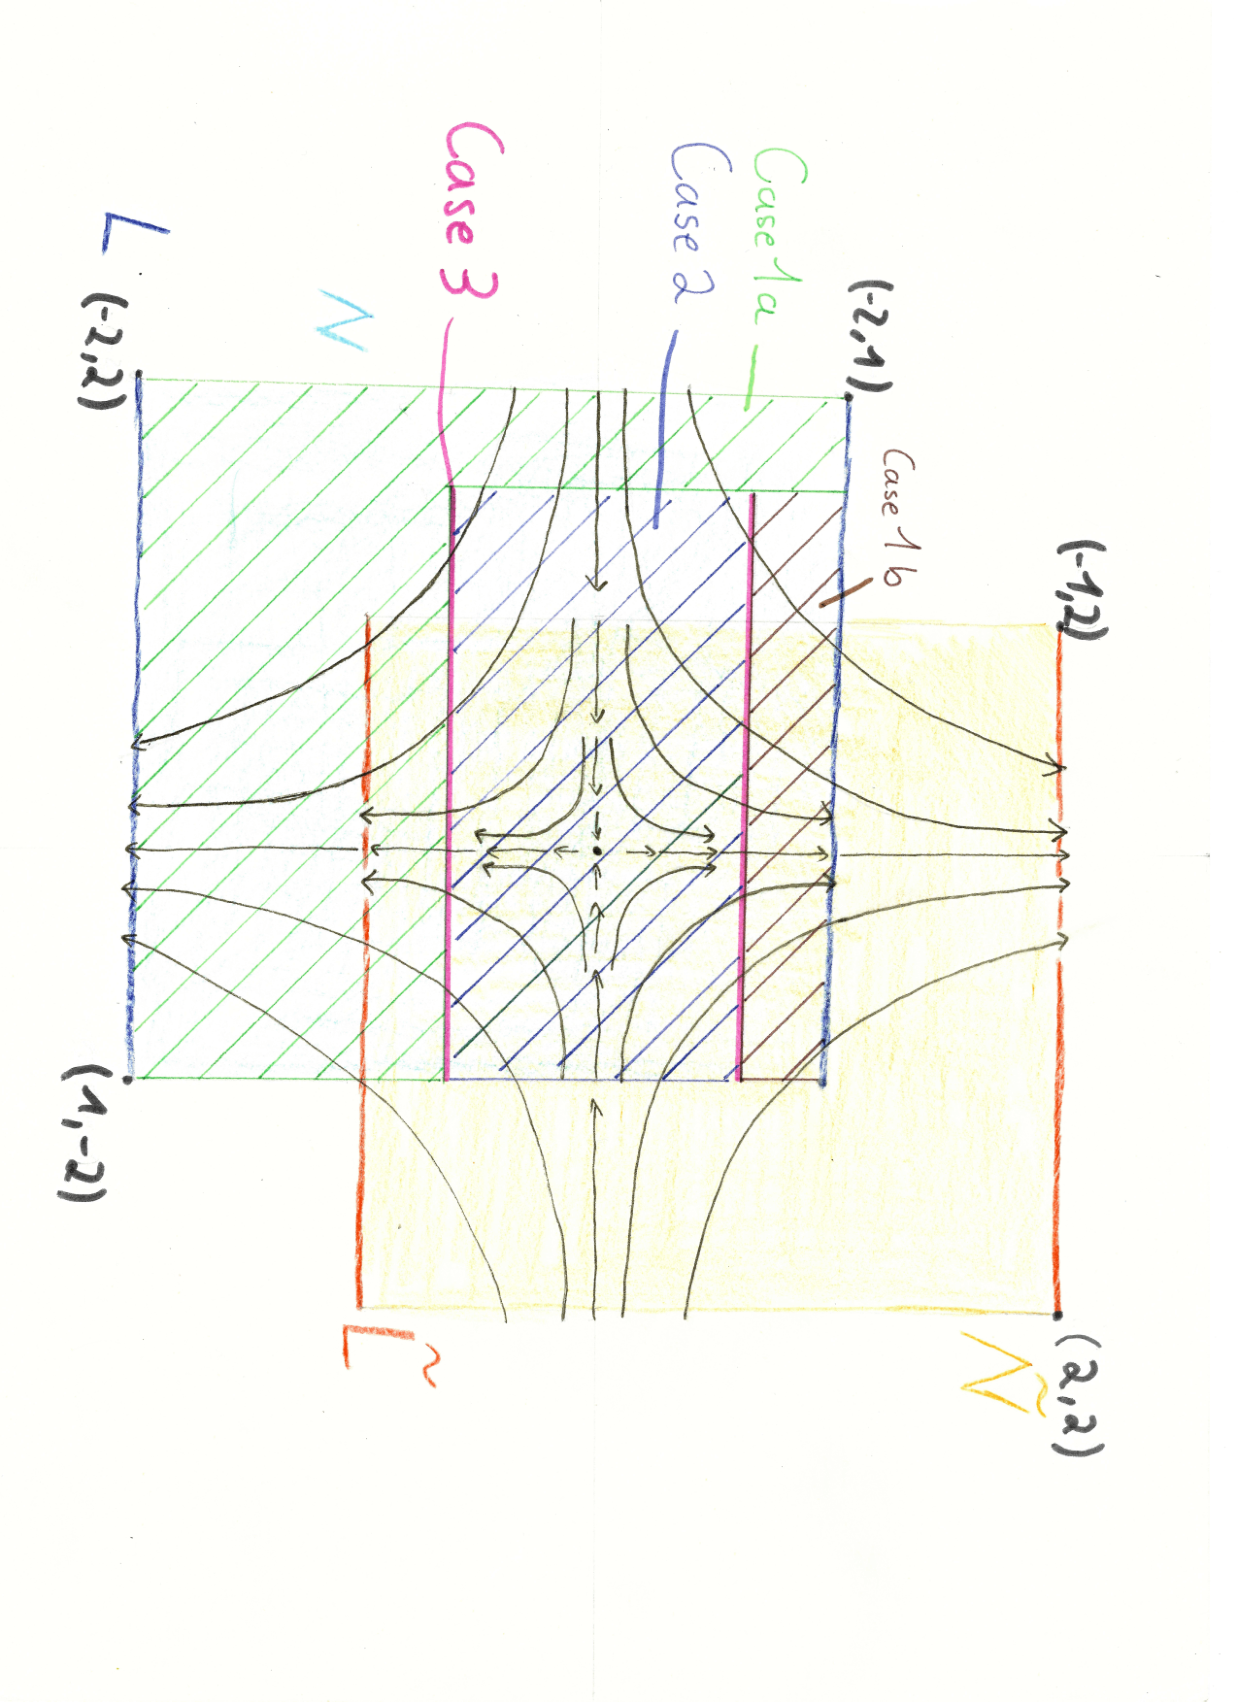
\includegraphics[angle=90,width=1\textwidth]{Text/Pictures/Index Pairs prove.pdf}
    \caption{The different cases for the proof of lemma \ref{lem: index invariants lemma 2}.}
    \label{fig: The different cases for the proof of lemma}
    In this picture the flow is induced by the vectorfield $(-x,y)$ and drawn for $t=\frac{1}{3}$. That is due to the ease of calculation and such that the four cases are all visible. In the picture $N=[-2,1]^2$ and $\tilde{N}=[-1,2]^2$. $L$ and $\tilde{L}$ are the horizontal borders. 
    \end{figure}\clearpage
    
\begin{proof}
We split this proof into three different cases that can be seen in figure \ref{fig: The different cases for the proof of lemma}. We always look at an image point lets say $h([x],t)$, choose an arbitrary neighbourhood $U$ and define a neighbourhood $W$ of $([x],t)$ such that the image of $W$ is contained in $U$. This clearly gives us locally $\epsilon-\delta-$continuity, as we are a metric space: 
\newline \textit{Case one a:} $\phi_{[t,3t]}(x)\not \subseteq \overline{\tilde{N}\setminus \tilde{L}}$. In this case there exists a ${t<t^*<3t}$ such that ${\phi_{t^*}(x)\nin \overline{\tilde{N}\setminus \tilde L}}$. $t^*$ can be taken strictly less then $3t$ since the complement of $\overline{\tilde{N}\setminus \tilde{L}}$ is open. Furthermore, this tells us the existence of a neighbourhood $U$ of $\phi_{t^*}(x)$ that is disjoint from $\overline{\tilde{N}\setminus \tilde{L}}$. And by the continuity of the flow we have a neighbourhood $W\subseteq M \times [T,\infty]$ such that $(x',t')\in W$ implies that $\phi_{t^*}(x')\in U$ and $t'<t^*<3t'$. Thus, $\phi_{[t',3t']}(x')\not \subseteq \tilde{N}\setminus \tilde{L}$ and therefore $h([x'],t')=[\tilde{L}]$ for all $(x',t')\in W$.

 We can argue the same way if $\phi_{[0,2t]} \not \subseteq  (N\setminus L)$ (\textit{Case one b}) and therefore conclude that in this case the map $h$ is continuous.
So for the rest of the proof we assume that we are in the first case of the map $h$ or at the boundary:
\begin{equation}
\phi_{[0,2t]}\subseteq \overline{N\setminus L} \text{ and } \phi_{[t,3t]}(x)\subseteq \overline{\tilde{N}\setminus \tilde{L}}. \label{eq: proof scnd lemma homotopy type independent case destinction}
\end{equation}
\newline \textit{Case two:} $\phi_{[t,3t]}(x)$ is disjoint with $\tilde{L}$. Then due to the closure of $\tilde{N}$ and (\ref{eq: proof scnd lemma homotopy type independent case destinction}) we can conclude that $\tilde{N}\setminus \tilde{L} \supseteq \phi_{[t,3t]}(x) = \phi_{[-t,t]}(\phi_{2t}(x))$ and by the implication (\ref{eq: lemma 2 2nd implic}) we can conclude that $\phi_{2t}(x) \in N\setminus L$. Since $L$ is the exit set we have that $\phi_{[0,2t]}(x)\subseteq N \setminus L$. By the above we have that $h([x],t)=[\phi_{3t}(x)]\in \tilde{N}\setminus \tilde{L}$. As before, due to the continuity of the flow we choose a neighbourhood $U$ of $\phi_{3t}(x)$ and find a neighbourhood $W\subseteq M \times [T,\infty)$ such that whenever $(x',t')\in W$ we have:
\begin{align*}
\phi_{[0,2t']}\cap L=\emptyset, \quad \phi_{[t',3t']}(x')\cap \tilde{L}=\emptyset, \quad \text{and} \quad \phi_{3t'}(x')\in U.
\end{align*}
If $x'$ is in $N$ then we have that $\phi_{[0,2t']}(x')$ is in $N\setminus L$ and similar to before we conclude with (\ref{eq: lemma 2 1st implic}) that $\phi_{t'}(x')\in \tilde{N}\setminus \tilde{L}$ and since $\tilde{L}$ is the exit set we have the inclusion ${\phi_{[t',3t']}(x')\subseteq \tilde{N} \setminus \tilde{L}}$. Therefore, we have that $h([x'],t')=[\phi_{3t'}(x')] \in U$ for all $(x',t')\in W$ where $x'\in N$. The continuity of the flow gives us continuity in this area.
\newline \textit{Case three:} $\phi_{[t,3t]}(x)$ intersects $\tilde{L}$. Then by (\ref{eq: proof scnd lemma homotopy type independent case destinction}) and since $\tilde{L}$ is the exit set we have that $\phi_{3t}(x)\in \tilde{L}$. 
Now define $[U]$ to be a neighbourhood of $h([x],t)=[\tilde{L}]$ in $\tilde{N}/\tilde{L}$. We want to find a representative of $[U]$, that is an open set of $M$ that reduces to $[U]$ in the quotient space. Let $\pi:\tilde{N}\to \tilde{N}/\tilde{L}$ be the quotient map. A natural choice would be 
$U\coloneq \pi^{-1}([U])$ which is without restriction open in $\tilde{N}$. To make it open in $M$ we can unite it with $M\setminus \tilde{N}$. Now again by the continuity of the flow we have an open neighbourhood $W\subseteq M\times [T,\infty)$ of $(x,t)$ such that whenever $(x',t')\in W$ we have that $\phi_{3t'}(x')\in U$. But then we have that:
\begin{align*}
h([x'],t')\in \{ [\phi_{3t'}(x')],[\tilde{L}] \} \subseteq [U] \cap [\tilde{L}]=[U].
\end{align*}
\end{proof}


\begin{lemma} \label{lem: index invariants lemma 3} Let $(N, L),(N',L')$ and $(\tilde{N},\tilde{L})$ be index pairs of $S$. Choose $T>0$ such that the implications (\ref{eq: lemma 2 1st implic}) and (\ref{eq: lemma 2 2nd implic}) are satisfied and furthermore choose a $\tilde{T}$ such that for $t> \tilde{T}$ we have:
\begin{align}
\phi_{[-t,t]}(x) \subseteq \tilde{N}\setminus \tilde{L} \quad & \Rightarrow \quad x\in N'\setminus L' \label{eq: lemma 3 1st implic} \\
\phi_{[-t,t]}(x) \subseteq N'\setminus L' \quad & \Rightarrow \quad x\in  \tilde{N}\setminus \tilde{L}.\label{eq: lemma 3 2nd implic} 
\end{align}
Now define:
\begin{align*}
h:N/L \times [T,\infty) & \to \tilde{N}/\tilde{L} \\
([x],t) & \mapsto 
\begin{cases}
[\phi_{3t}(x)] & \text{ if } \phi_{[0,2t]}\subseteq N\setminus L \text{ and } \phi_{[t,3t]}(x)\subseteq \tilde{N}\setminus \tilde{L}\\
[\tilde{L}] & \text{ otherwise,}
\end{cases}
\end{align*}
and 
\begin{align*}
\tilde{h}:\tilde{N} / \tilde{L} \times [\tilde{T},\infty) & \to N'/L' \\
([x],t) & \mapsto 
\begin{cases}
[\phi_{3t}(x)] & \text{ if } \phi_{[0,2t]}\subseteq \tilde{N} \setminus \tilde{L} \text{ and } \phi_{[t,3t]}(x)\subseteq N'\setminus L'\\
[L'] & \text{ otherwise.}
\end{cases}
\end{align*} 
Then the following equations hold for $t\geq \max\{T,\tilde{T}\}$:
\begin{equation*}
\tilde{h}\big(h([x],t),t\big)=
\begin{cases}
[\phi_{6t}(x)] & \text{if }\phi_{[0,4t]}\subseteq N\setminus L \text{ and } \phi_{[2t,6t]}(x)\subseteq N'\setminus L' \\
[L'] &\text{otherwise.}
\end{cases}
\end{equation*}
\end{lemma}
\begin{proof}
The proof is just the equivalence of the two statements:
\begin{align*}
& \phi_{[0,4t]}\subseteq N\setminus L \text{ and } \phi_{[2t,6t]}(x)\subseteq N'\setminus L' \\
\Leftrightarrow \quad & \phi_{[0,2t]}(x)\subseteq N\setminus L,~ \phi_{[t,5t]}(x)\subseteq \tilde{N}\setminus \tilde{L},~\phi_{[4t,6t]}(x)\subseteq N' \setminus L'.
\end{align*}
\newline \glqq $\Rightarrow$\grqq~ Here we need to check three things. The first and the third inclusion are trivially satisfied. For the second we notice that $\phi_{[0,4t]}\subseteq N\setminus L$ implies that $\phi_{[t,3t]}(x)\subseteq \tilde{N} \setminus \tilde{L}$ by implication (\ref{eq: lemma 2 1st implic}). Furthermore, $\phi_{[2t,6t]}(x)\subseteq N'\setminus L'$ implies that $\phi_{5t}(x)\in \tilde{N}\setminus \tilde{L}$ by implication (\ref{eq: lemma 3 2nd implic}). And since $\tilde{L}$ is the exit set this implies the missing second inclusion.
\newline \glqq $\Leftarrow$\grqq~ For the first inclusion notice that $x=\phi_0(x)\in N$ by definition and $\phi_{[t,5t]}(x)\subseteq \tilde{N}\setminus \tilde{L}$ implies $\phi_{[2t,4t]}(x)\subseteq N \setminus L$ by implication (\ref{eq: lemma 2 2nd implic}). Using the exit set property we conclude that $\phi_{[0,4t]}\subseteq N\setminus L$. Finally, $\phi_{[t,5t]}(x)\subseteq \tilde{N}\setminus \tilde{L}$ implies that $\phi_{[2t,4t]}(x)\subseteq N' \setminus L'$ by (\ref{eq: lemma 3 1st implic}).

Together with $\phi_{[4t,6t]}(x)\subseteq N' \setminus L$ this lets us conclude that $ \phi_{[2t,6t]}(x)\subseteq N'\setminus L'$. The additive property of the flow does the rest letting us conclude that we are in the first case of $h$ and $h'$ if and only if the stated property is satisfied.  
\end{proof}

\begin{theorem}[Homotopy equivalence of index pairs] \label{thm: Homotopy equivalence of index pairs}
If $S$ is an isolated compact invariant set and $(N,L)$ and $(\tilde{N},\tilde{L})$ are two index pairs of $S$. Then $N/L$ and $\tilde{N}/\tilde{L}$ are homotopy equivalent as pointed spaces.
\end{theorem}
\begin{proof}
Let $h_t:N/L \to \tilde{N}/ \tilde{L}$ and $g_t:\tilde{N}/\tilde{L}\to N/L$ be the continuous family of maps from lemma \ref{lem: index invariants lemma 2}. By lemma \ref{lem: index invariants lemma 3} we get that
\begin{align*}
g_t\circ h_t([x])=
\begin{cases}
[\phi_{6t}(x)] & \text{if }\phi_{[0,4t]}\subseteq N\setminus L \text{ and } \phi_{[2t,6t]}(x)\subseteq N\setminus L \\
[L] &\text{otherwise.}
\end{cases}
\end{align*} 
Furthermore, we use lemma \ref{lem: index invariants lemma 2} for $T=0$.
And now we can explicitly write down a homotopy from the identity to $g_t\circ h_t([x])$ as follows:
\begin{align*}
H: N/L \times [0,1] &\to N/L\\
([x],t')&\mapsto \begin{cases}
[\phi_{6t't}(x)] & \text{if }\phi_{[0,4t't]}\subseteq N\setminus L \text{ and } \phi_{[2t't,6t't]}(x)\subseteq N\setminus L  \\
[L] & \text{otherwise.}
\end{cases}
\end{align*}
This homotopy is continuous by lemma \ref{lem: index invariants lemma 2} and $H(\cdot,0)=\id$ and $H(\cdot,1)=g_t\circ h_t$. Similar we show that $h_t\circ g_t $ is homotopic to the identity. With this we have that
\begin{align*}
N/L ~ \simeq \tilde{N}/\tilde{L} .
\end{align*}
\end{proof}

\begin{definition}[The homotopy Conley index]
The \textbf{Conley index} of an invariant set $S$ is defined as $\pi_1(N,L)$ where $(N,L)$ is a regular index pair. This definition is invariant of the chosen pair and is an invariant of invariant sets. 
\end{definition}
\section{A Morse Theoretic Filtration}
In this subchapter we will finally prove the Morse homology theorem. We start by defining some index sets that we will later use in the prove. Again, this prove is due to Solomon and found in \cite{MorseTheorySalmbon}.

\begin{example}[Critical points as isolated compact invariant subsets] \label{ex: Critical points as isolated compact invariant subsets}
    Let ${f:M\to \R}$ be a Morse function on a smooth Riemannian manifold $(M,g)$. Let $q\in \Crit_k(f)$. Around $q$ we have coordinate charts $\phi:U \to T_qM$ (after identifying $q_i$ and $\partial q_i$) where  ${\phi(W(q\to)\cap U)\subseteq T_q^{u}M}$ and ${\phi(W(\to q)\cap U)\subseteq T_q^{s}M}$. With this we can define the balls:
    \begin{align*}
        D^{s}_\epsilon &~=~\{v\in T_q^{s}M | \norm{v}\leq \epsilon \}, \\
             D^{u}_\epsilon &~=~\{v\in T_q^{u }M | \norm{v}\leq \epsilon \}. 
    \end{align*} They give rise to the index pair $N_q\coloneq\phi^{-1}( D^{s }\times  D^{u })$ and $L_q=\phi^{-1}( D^{ s}\times \partial D^{u})$. This index pair is in fact regular, since $(N_q,L_q)\cong  (D^{ s}\times  D^{u }, D^{s}\times \partial D^{u}) \cong (D^{u}_{\epsilon},\partial D^{u}_{\epsilon} )$. Now we can make the first step towards singular homology, since we know the homology  of such a tuple:
    \begin{align} \label{eq: homology of indexx pair of critical point}
        H^{\sing}_i(N_q,L_q)=H^{\sing}_i(D^{k},\partial D^{k})=\begin{cases}
            \Z & \text{if } i=k,\\
            0& \text{else. }
        \end{cases}
    \end{align}
    Notice that for $k=0$ we need to consider $\partial D^k=\emptyset$, to get an index pair. That's why we let $\partial$ denote the manifold boundary insted of the topological boundary. However, now we can identify for all $k$: \begin{equation} \label{ kritical points as direct sum of homology groups}
        C_k(M,f)=\bigoplus_{ \Crit_k(f)} \Z \cong \bigoplus_{q\in \Crit_k(f)} H_k(N_q,L_q;\Z).
    \end{equation}
    Furthermore, this isomorphism can be made canonically, by using orientations: Notice for this that $(N_q/L_q)$ is homotopic equivalent to $W(q\to)/ (W(q \to)\setminus \{q\})$. Here we get a generator of the $ k-$homology group induced by an orientation on $T^u_pM$ that then canonically maps to the $k-$th homology group of $(N_q,L_q)$.
\end{example}

\begin{example}[A map of homology groups]
     Let $f:M\to \R$ be a Morse Smale function on a smooth compact Riemannian manifold $(M,g)$. Let $q\in \Crit_k(f)$ and $p\in \Crit_{k-1}(f)$. Assume for a moment we already have an isolated regular compact index pair $(N_2,N_0)$ of $S=W(p\to q)\cup\{p,q\}$. 
     For a $c\in (f(p),f(q))$ we set $N_1=N_0\cup (N_2 \cap M^c)$ depicted in figure \ref{fig: Gradient flow lines as isolated compact invariant sets}, where $M^c$ is the sublevel set. Clearly now $(N_2,N_1)$ is an index pair for $q$ and $(N_1,N_0)$ is a pair for $p$. Assuming we have regular index pairs $(N_q.L_q)$ and $(N_p,L_p)$ for $p,q$ we can now define a map:
     \begin{align*}
         \Delta_k(q \to p): H^{\sing}_k(N_q,L_q) \to H^{\sing}_{k-1}(N_p,L_p)
     \end{align*} as the composition:
\begin{center}
   % https://tikzcd.yichuanshen.de/#N4Igdg9gJgpgziAXAbVABwnAlgFyxMJZABgBpiBdUkANwEMAbAVxiRAAkB9AawAoA5TgEdSAGWEBuADpSAWgEoQAX1LpMufIRQBGclVqMWbLn0EAmUoO3S5ilWux4CRC5Wr1mrRB07BuAWm0lAU5dQWIbBWVVEAxHTSIAZj13Qy8fP0DgwTQxTjRIu30YKABzeCJQADMAJwgAWyQyEBwIJF0DTzYZAGMCUujqusbECxa2xGTOo29e-sGQWob26lakMY8ZkBlYBhw6HmUKJSA
\begin{tikzcd}
{H_k(N_q,L_q;\Z)} \arrow[r, "\cong"] & {H_k(N_2,N_1)} \arrow[r, "\delta_*"] & {H_{k-1}(N_1,N_0)} \arrow[r, "\cong"] & {H_{k-1}(N_p,L_p)}
\end{tikzcd}
\end{center} where $\delta_*$ is the connecting homomorphism, and the other two maps are induced by the homotopic equivalence of two index pairs corresponding to the same isolated compact invariant subset. Putting all together we can define a morphism:
\begin{align}\label{equation: definition of boundary operator for filtrations}
    \Delta_k:\bigoplus_{q\in \Crit_k(f)}H^{\sing}_k(N_q,L_q)\to \bigoplus_{p\in \Crit_{k-1}(f)}H^{\sing}_{k-1}(N_p,L_p).
\end{align}
\end{example}

\begin{figure}[p!]
    \centering
    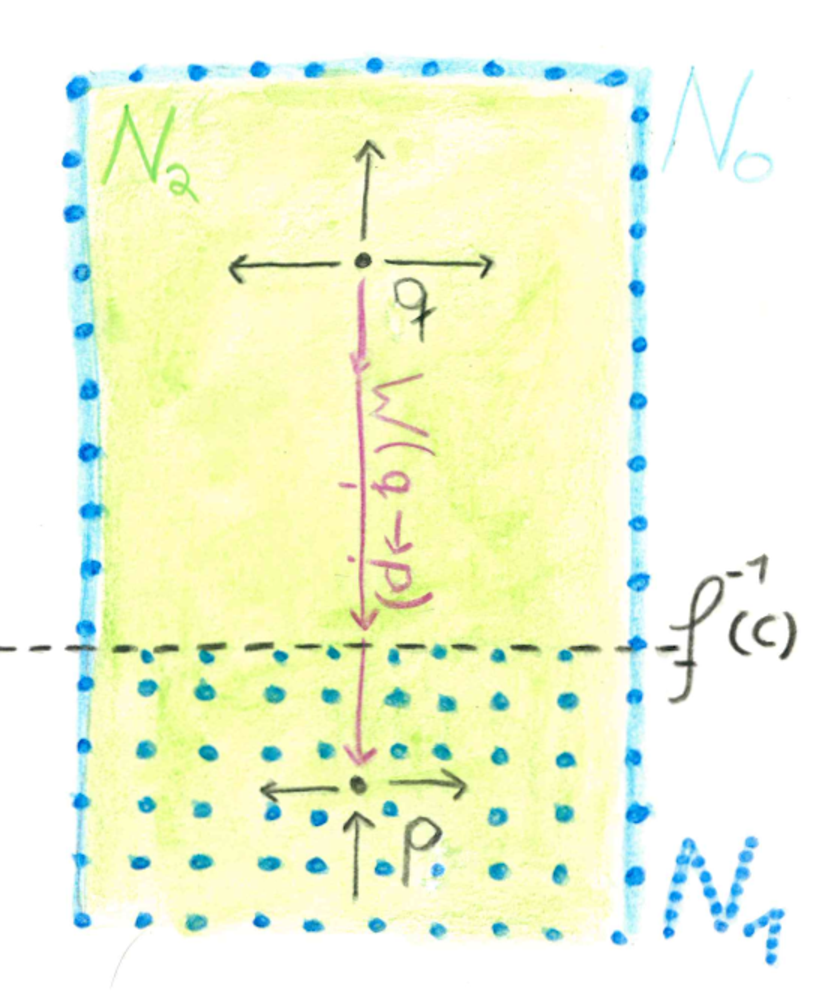
\includegraphics[width=0.5\linewidth]{Text/Pictures/definitionN_1.pdf}
    \caption{Index pairs for gradient flow lines.}
    \label{fig: Gradient flow lines as isolated compact invariant sets}
\end{figure}\clearpage










































\begin{definition}[Regular index pairs and a filtration on $M$] \label{def: Regular index pairs and a filtration on M } \label{def: Regular index pairs and a filtration on M}
As always let $f:M\to \R$ be a Morse-Smale function on a compact smooth Riemannian manifold $(M,g)$ of dimension $m$. Let $\phi_t:M\to M$ be the flow given by $-\grad f$. For $0\leq j\leq k\leq m$ define:
\begin{align*}
    W(k,j)=\bigcup_{j\leq \lambda_p \leq \lambda_q\leq k} W(q \to p).
\end{align*}We know that this space is compact\todo{reference}. Assume that $N$ is a compact neighbourhood of $W(k,j)$, such that $\Crit(f)\cap N=\Crit(f)\cap W(k , j)$, meaning that $N$ does not contain any new critical points. Then the biggest invariant subspace from definition \ref{def: index pairs} is
\begin{align*}
    I(N)\coloneq\{x\in N| \phi_t(x)\in N \forall t \in \R \}=W(j,k).
\end{align*} This follows from every gradient flow line starting and ending in a critical point.  Therefore, $W(k,j)$ is an isolated compact invariant set. By a corollary of the lambda lemma \todo{reference} we know that 
\begin{align*}
    W^{s}_{j}&~\coloneq~ \bigcup_{j\leq \lambda_p}W(\to p)\\
    W^{u}_{ j}&~\coloneq~\bigcup_{\lambda_p\leq j}W(p \to )
\end{align*}for all $j=0,...,m$ are compact as they are finite unions of compact sets. Now we define $N_m\coloneq M$ and choose a cofibered compact neighbourhood $N_{m-1}$ of $W^{p\to }_{m-1}$ that is positively invariant and satisfies $N_{m-1}\cap W^{\to p}_m=\emptyset$
One could for example define:
\begin{align*}
    N_{m-1}\coloneq N_m \setminus \Big(\bigcup_{q\in \Crit_m(f)}  \mathring{N_q}\Big),
\end{align*} where $N_q$ is taken from example \ref{ex: Critical points as isolated compact invariant subsets}. Once we check that $N_{m-1}$ is an exit set with respect to $N_m$ we can conclude that $(N_m,N_{m-1})$ is a regular index pair for $\Crit_m(f)$. The first statement is clear, since every gradient line starting in $N_m\setminus N_{m-1}$ has to pass through $N_{m-1}$, as they go towards other critical points. This tells us that they have to leave $N_m\setminus N_{m-1}$, which is enclosed by $N_{m-1}$. The second thing to check can be done by showing that there is a neighbourhood $U\subset N_M$ of $N_{m-1}$ that deforms to $N_{m-1}$. For this notice that each $N_q$ with $\lambda_q=m$ is homeomorphic to $D^m$. Now choose a open neighbourhood $U_q$ in the disc of its boundary. By definition this retracts to the boundary with a retraction induced by the flow. And finally define $U\coloneq N_{m-1}\cap_{q\in \Crit_m(f)} U_q$. This retracts to $N_{m-1}$ telling us that our index pair is indeed regular. 

Now we want to inductively define a filtration: 
For this we choose a compact cofibered neighborhood $N_{m-2}$ of $W^{u}_{m-2}$ that is positifely invariant in $N_{m-1}$ and has an empty intersection with $W^{\to p}_{m-1}$. This can be done similar to the construction of $N_{m-1}$ but instead of cutting out neighbourhoods if $q\in \Crit_{m}(f)$, we can cut out tubular neighborhoods of $W^{s}_{m-1}$. This is depicted in figure \ref{fig: Definition of the filtration} for the torus. By iterating this process we get a filtration: 
\begin{equation} \label{eq: Filtration conley}
    \emptyset=:N_{-1}\subset N_0\subset N_1\subset \cdots \subset N_{m-1}\subset N_m=M,
\end{equation} such that $(N_k,N_{j-1})$ is a regular index pair for $W(k,j)$ for all $0\leq j \leq k\leq m$.
\end{definition}
\begin{figure}[p!]
    \centering
    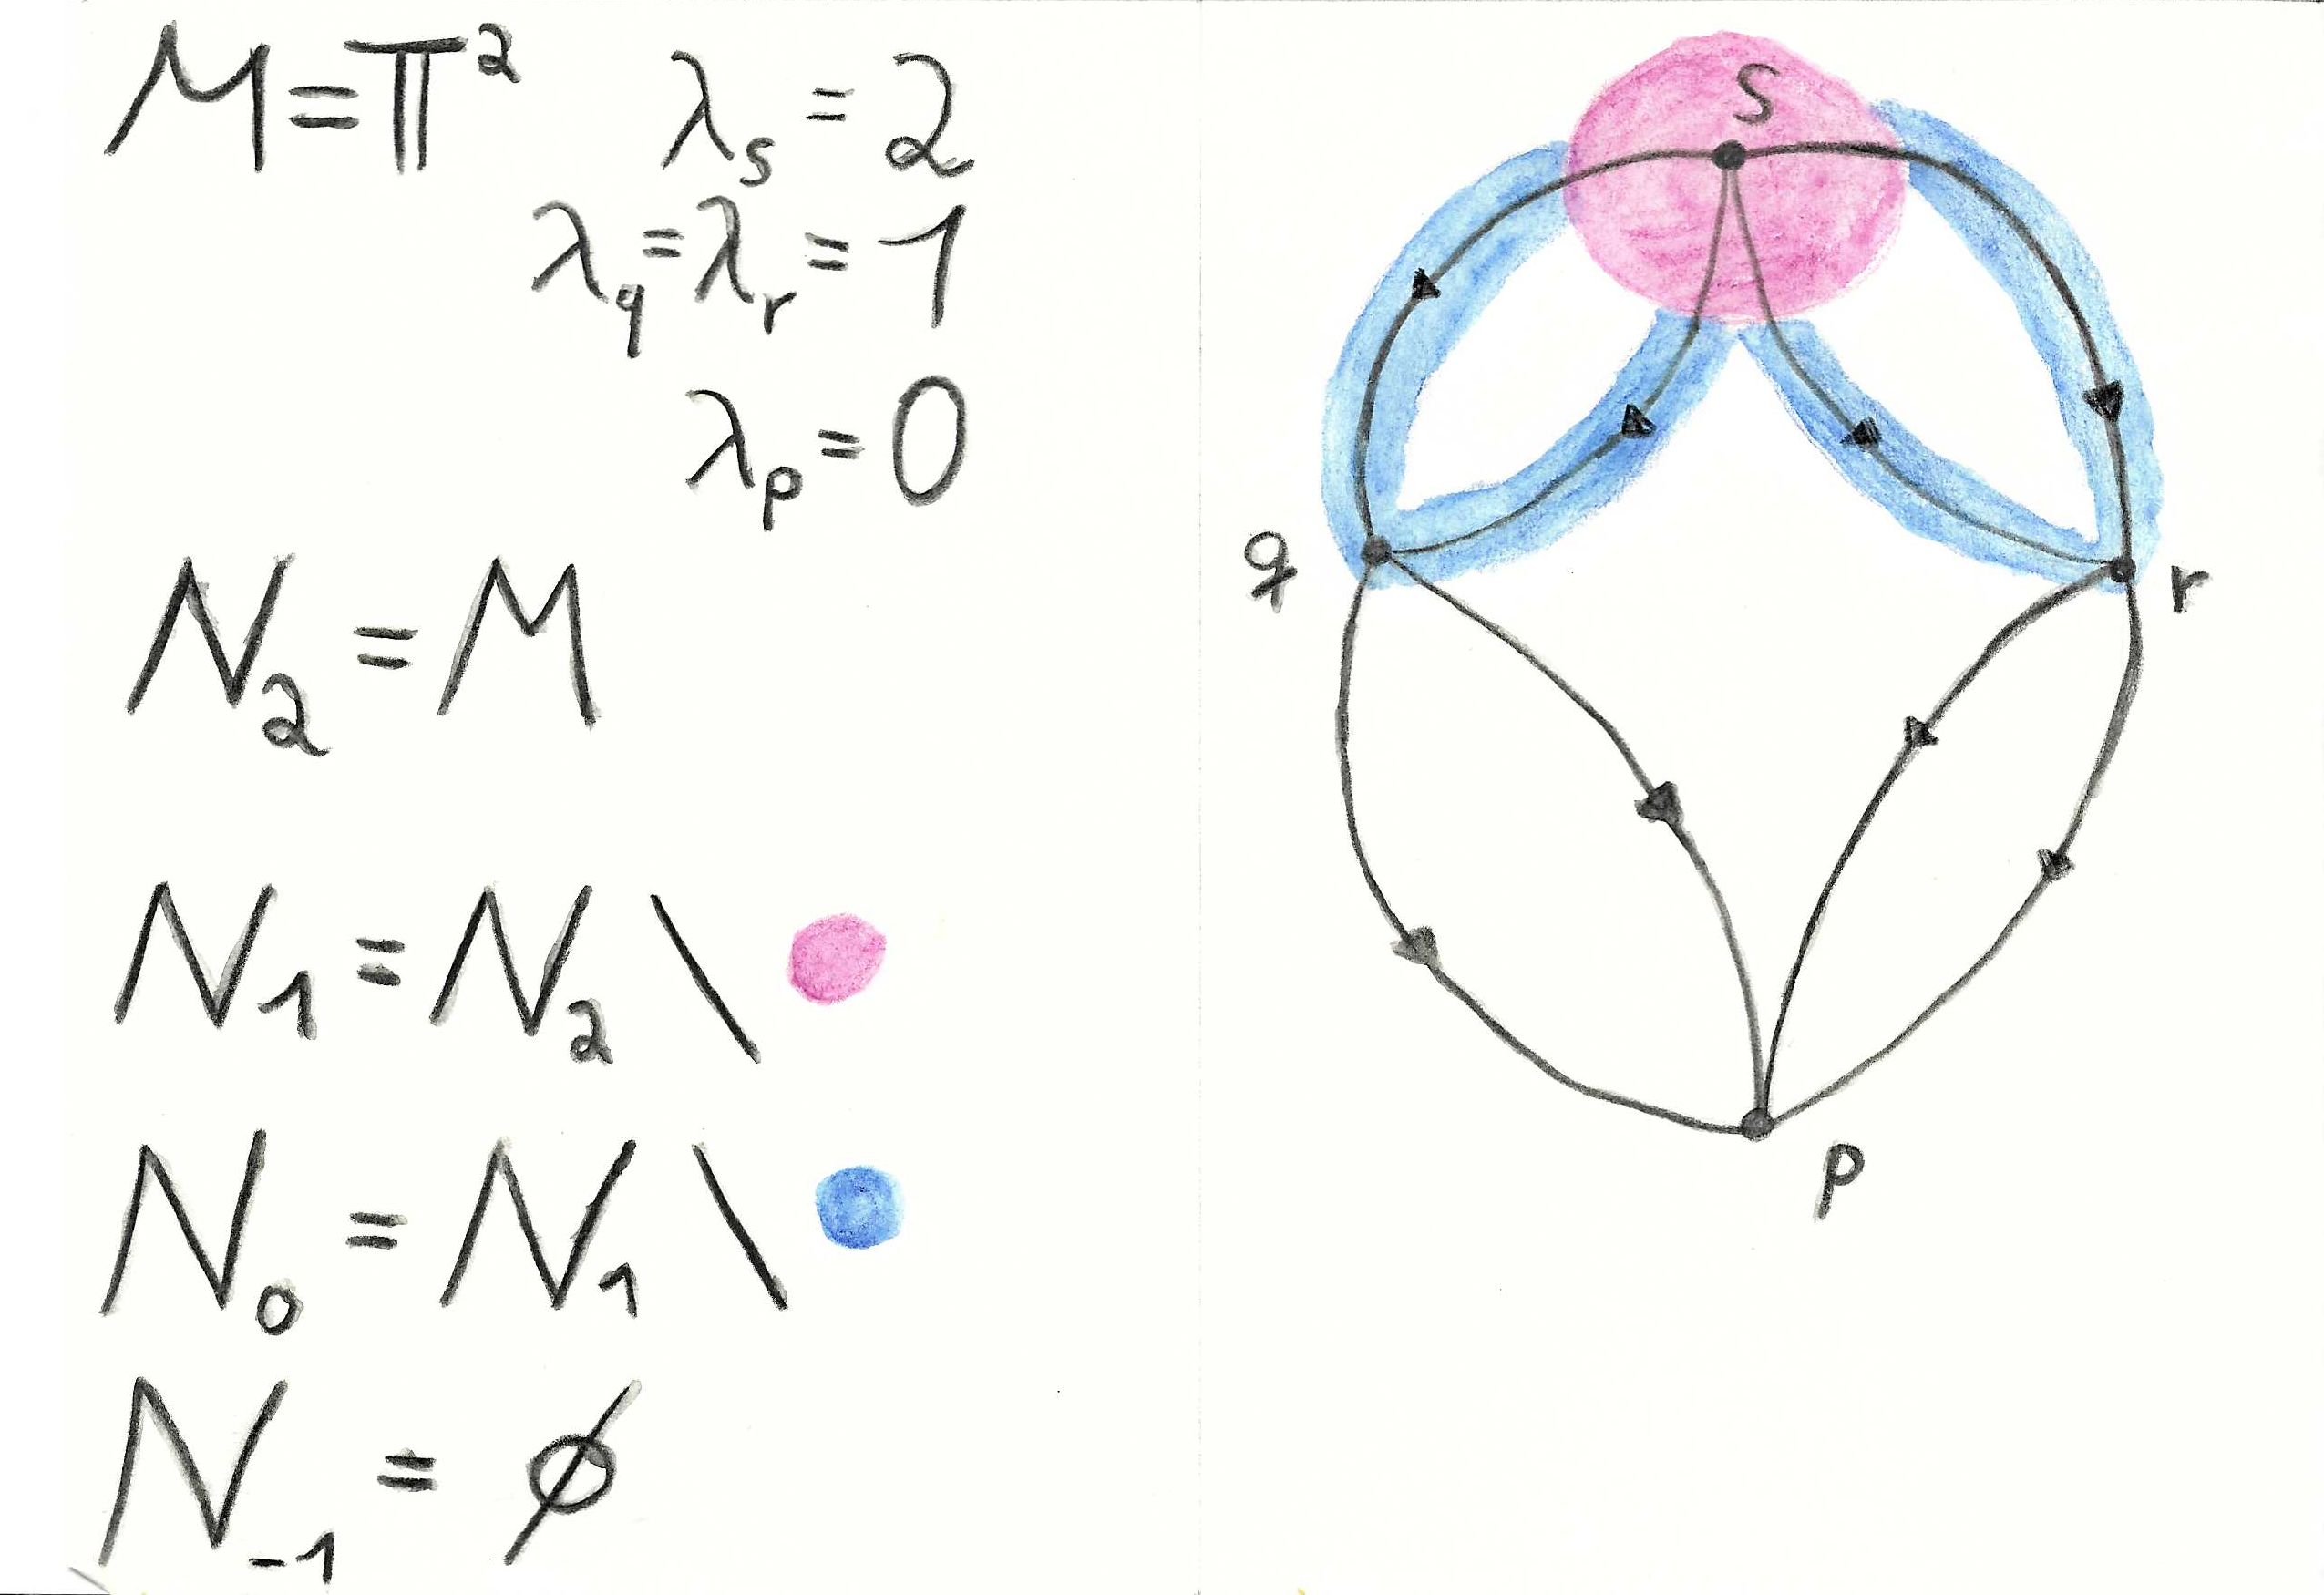
\includegraphics[width=0.5\textwidth]{Text/Pictures/Filtration.png}
    \caption{The filtration of the torus.}
    \label{fig: Definition of the filtration}
The picture shows the phase diagram of the torus and schematically depicts the filtration. 
\end{figure}\clearpage
